\documentclass[../ecuaciones_diferenciales.tex]{subfiles}

\begin{document}
Hasta ahora nos hemos preocupado de \emph{resolver} los sistemas de ecuaciones
diferenciales lineales. Ahora queremos entender el comportamiento
\emph{cualitativo} de sus soluciones.

Haciendo una analogía con el análisis real, un planteamiento cuantitativo es
tener una fórmula explícita para una función y uno cualitativo es dar la forma
global de su gráfica (crecimiento, convexidad, asíntotas...)

Si sabemos resolver explícitamente los sistemas, ¿por qué interesa hacer un
análisis cualitativo?

\begin{enumerate}[1)]
	\item En muchos casos, nos da información relevante del modelo estudiado. Por
	      ejemplo, es importante saber si una enfermedad desaparece o se hace endémica,
	      si una población oscila, se estabiliza o desaparece, si un tumor crece sin
	      control o su crecimiento se termina estabilizando, si las oscilaciones de un
	      puente acabarán pasando el umbral de rotura, etc.

	\item En el caso no lineal, esto es esencialmente lo único que se puede decir
	      (aparte de dar aproximaciones numéricas de la solución).
\end{enumerate}

Nos centraremos exclusivamente en \emph{sistemas planos} (matrices \(2 \times 2\))
y en el caso homogéneo de coeficientes constantes, es decir, en sistemas de la
forma
\[x' = Ax, \qquad A = \mat{a_{11} & a_{12} \\ a_{21} & a_{22}}.\]
Estamos interesados en pintar las trayectorias u órbitas:

\begin{definition}
	Dada una solución \((x_1(t), x_2(t))\) de un sistema \(x' = Ax\), su
	\emph{trayectoria} u \emph{órbita} es el conjunto
	\(\{(x_1(t), x_2(t)) : t \in \R\} \subset \R^2\).
\end{definition}

\begin{definition}
	El conjunto de todas las trayectorias de \(x' = Ax\) se llama \emph{diagrama
		de fases} del sistema.
\end{definition}

\begin{example}\label{ex:fases_1}
	Dibujar el diagrama de fases del sistema \(x' = Ax\) siendo
	\(A = \smat{0 & 1 \\ -1 & 0}\).

	Como ya vimos, la solución general viene dada por
	\[\eqsys{
			x_1(t) = k_1 \cos t + k_2 \sin t \\
			x_2(t) = - k_1 \sin t + k_2 \cos t}\]

	Nuestro objetivo es eliminar \(t\) de estas ecuaciones para obtener la
	relación entre \(x_1\) y \(x_2\) que define la trayectoria.

	La solución se puede escribir como

	\[\mat{x_1 \\ x_2} = e^{At}\mat{k_1 \\ k_2} =
		\underbrace{\mat{\cos t & \sin t \\ -\sin t & \cos t}}_{\text{matriz de
				rotación}} \mat{k_1 \\ k_2},\]

	así que, intuitivamente, la trayectoria es una circunferencia que pasa por
	\(\smat{k_1 \\ k_2}\). Analíticamente,
	\begin{align*}
		x_1^2 + x_2^2 & = (k_1^2\cos^2t + k_2^2\sin^2t + 2k_1k_2\cos t \sin t)
		+ (k_1^2\sin^2t + k_2^2\cos^2t - 2k_1k_2\cos t \sin t)                                 \\
		              & = k_1^2(\cos^2 t + \sin^2 t) + k_2^2(\cos^2t + \sin^2t) = k_1^2+k_2^2.
	\end{align*}
	Efectivamente, la trayectoria que pasa por \(\smat{k_1 \\ k_2}\) es la
	circunferencia centrada en el origen de radio \(\sqrt{k_1^2+k_2^2}\). Además,
	conforme \(t\) aumenta, la trayectoria se recorre en sentido horario.
\end{example}

\begin{figure}[ht]
	\centering
	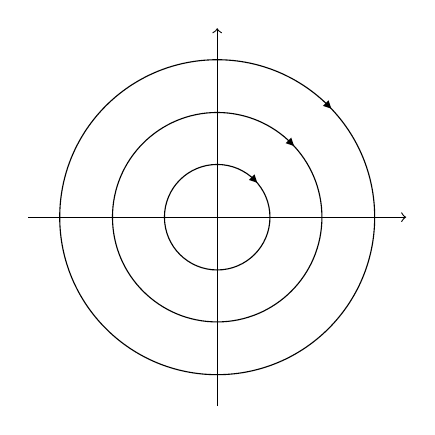
\begin{tikzpicture}
		\draw[->] (-2.4,0) -- (2.4,0);
		\draw[->] (0,-2.4) -- (0,2.4);
		\draw (0,0) circle (0.67);
		\fill[rotate=45] (0.67,-0.05) -- (0.72, 0.05) -- (0.62, 0.05) -- cycle;
		\draw (0,0) circle (1.33);
		\fill[rotate=45] (1.33,-0.05) -- (1.38, 0.05) -- (1.28, 0.05) -- cycle;
		\draw (0,0) circle (2.00);
		\fill[rotate=45] (2.00,-0.05) -- (2.05, 0.05) -- (1.95, 0.05) -- cycle;
	\end{tikzpicture}
	\caption{Diagrama de fases del sistema del ejemplo~\ref{ex:fases_1}}
\end{figure}


\begin{theorem}
	Las trayectorias no se cortan.
	\begin{proof}
		Supongamos que las trayectorias asociadas a las soluciones \(x(t), y(t)\) de
		\(x' = Ax\) se cortan o, en otras palabras, que existen \(t_1, t_2\) tales
		que \(x(t_1) = y(t_2)\). Lo que ocurre es que \(y(t) = x(t + (t_1-t_2))\),
		luego la trayectoria que definen ambas soluciones resulta ser la misma.

		Para ver esto, definimos \(z(t) = x(t + (t_1-t_2))\). Se cumple que \(z' =
		Az\) y \(z(t_2) = x(t_1) = y(t_2)\), luego, en virtud del teorema de
		existencia y unicidad, debe ser \(z(t) = y(t)\).
	\end{proof}
\end{theorem}

\begin{remark}
	Ya vimos que las gráficas de \(x(t), y(t)\) no se cortan (como subconjuntos de
	\(\R^3\)). Este resultado, más fuerte, quiere decir que no se cortan \emph{sus
		proyecciones}, y se cumple porque \(A\) tiene coeficientes constantes (en
	caso contrario, no sería necesariamente cierto que \(z' = Az\)).
\end{remark}

\section{Interpretación geométrica de las trayectorias}

Una matriz \(A\), o más precisamente su aplicación lineal asociada \(A : \R^2
\to \R^2,\ x \mapsto Ax\), es un \emph{campo vectorial}. Una solución del
sistema \(x' = Ax\) no es más que una curva \(t \mapsto x(t)\) tal que su
velocidad \(x'(t)\) coincide con el valor del campo en \(x(t)\), es decir, una
\emph{curva integral} del campo.

\begin{example} \label{ex:campo_vec}
	Sea la matriz \(A = \smat{0 & 1 \\ -1 & 0}\). Esbozar el campo vectorial que
	define.

	La matriz \(A\) actúa sobre un vector genérico \(\smat{x_1 \\ x_2}\) como
	\(\smat{x_1 \\ x_2} \mapsto A\smat{x_1 \\ x_2} = \smat{x_2 \\ -x_1}\).
	Observamos que \(\langle x, Ax \rangle = 0\), es decir, la velocidad es
	ortogonal a la posición en todo punto, y además \(\|x\| = \|Ax\|\), es decir,
	\(A\) no cambia la norma de los vectores. El campo vectorial que define esta
	matriz es, entonces,
\end{example}

\begin{figure}[ht]
	\centering
	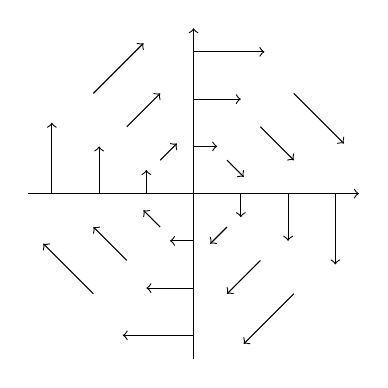
\begin{tikzpicture}[scale=0.6]
		\draw[->] (-3.5,0) -- (3.5,0);
		\draw[->] (0,-3.5) -- (0,3.5);
		\foreach \r in {1, 2, 3}
		\foreach \a in {0,...,7}
		\draw[->] ({\r*cos(45*\a)}, {\r*sin(45*\a)}) --
		({\r*cos(45*\a)+\r/2*sin(45*\a)}, {\r*sin(45*\a)-\r/2*cos(45*\a)});
	\end{tikzpicture}
	\caption{Campo vectorial generado por la matriz del
		ejemplo~\ref{ex:campo_vec}}
\end{figure}

\section{Representación gráfica de los sistemas planos}

Nos centramos ahora en esbozar el diagrama de fases de un sistema plano general
\(x' = Ax\), siendo \(B = P^{-1}AP\) su forma de Jordan. El cambio de variable
\(y = P^{-1}x\) transforma el sistema \(x' = Ax\) en \(y' = By\), mucho más
manejable. Las formas de Jordan posibles son

\begin{multicols}{2}
\begin{enumerate}[a)]
	\item \(B = \smat{\lambda_1 & \\ & \lambda_2},\ \lambda_1 \neq \lambda_2\)
	\item \(B = \smat{\lambda & \\ & \lambda}\)
	\item \(B = \smat{\lambda & 1 \\ & \lambda}\)
	\item \(B = \smat{a & b \\ -b & a},\ b>0\)
\end{enumerate}
\end{multicols}

Haremos los diagramas de fase para las formas de Jordan, y luego desharemos el
cambio de variable para obtener el diagrama final.

\subsection{Diagonalizable con dos autovalores reales distintos}

Consideramos el sistema \(y' = \smat{\lambda_1 & \\ & \lambda_2} y\), con
\(\lambda_1 \neq \lambda_2\). Como hemos visto, la solución general del sistema
es
\[\eqsys{
	y_1 = k_1e^{\lambda_1 t} \\
	y_2 = k_2e^{\lambda_2 t}}\]

Vamos a fijar distintos valores de \(k_1,k_2\) (i.e. distintos valores
iniciales) para ver cómo evoluciona el sistema a partir de ellos.

Empezamos por fijar valores sencillos, en los que algún valor inicial es 0
(valores iniciales en algún eje de coordenadas):
\begin{itemize}
	\item \(k_1 = 0, k_2 = 0\): en este caso, la trayectoria es \(\{(0,0)\}\). Como
	      consiste en un único punto, que permanece estable a lo largo del tiempo, se
	      llama \emph{punto de equilibrio}.

	\item \(k_1 > 0, k_2 = 0\): la trayectoria es \(\{(k_1e^{\lambda_1 t}, 0) : t \in
	      \R\} = \{(y_1, 0) : y_1 > 0\}\)

	\item \(k_1 < 0, k_2 = 0\): la trayectoria es \(\{(k_1e^{\lambda_1 t}, 0) : t \in
	      \R\} = \{(y_1, 0) : y_1 < 0\}\)

	\item \(k_1 = 0, k_2 > 0\): la trayectoria es \(\{(0, k_2e^{\lambda_2 t}) : t
	      \in \R\} = \{(0,y_2) : y_2 > 0\}\)

	\item \(k_1 = 0, k_2 < 0\): la trayectoria es \(\{(0, k_2e^{\lambda_2 t}) : t
	      \in \R\} = \{(0,y_2) : y_2 < 0\}\)
\end{itemize}

En general, la trayectoria que pasa por el punto \(\smat{k_1 \\ k_2} \in \R^2\),
no necesariamente en algún eje, es
\(\{(k_1e^{\lambda_1 t}, k_2e^{\lambda_2 t}) : t \in \R\}\). Si el punto no está
sobre ninguno de los ejes, se cumple \(k_1 \neq 0 \neq k_2\), con lo que se
puede dividir entre ellos. Elevando la primera coordenada a \(\lambda_2\) y la
segunda a \(\lambda_1\), se tiene
\begin{equation}\label{eq:impl}
	\begin{cases}
		y_1^{\lambda_2} = k_1^{\lambda_2}e^{\lambda_1\lambda_2 t} \\
		y_2^{\lambda_1} = k_2^{\lambda_1}e^{\lambda_1\lambda_2 t}
	\end{cases} \implies \left(\frac{y_1}{k_1}\right)^{\lambda_2} = e^{\lambda_1
			\lambda_2 t} = \left(\frac{y_2}{k_2}\right)^{\lambda_1}.
\end{equation}

Como \(\lambda_1 \neq \lambda_2\), alguno de los dos tiene que ser distinto de
0; podemos suponer, sin pérdida de generalidad, que es \(\lambda_1\). Despejando
en \eqref{eq:impl}, llegamos a
\[y_2 = k_2 \left(\frac{y_1}{k_1}\right)^{\lambda_2 / \lambda_1}\]
es decir, una relación de la forma \(y_2 = c y_1^\alpha\). Distinguimos casos en
función del valor de \(\alpha\):

\begin{figure}[ht]
	\centering
	\begin{subfigure}{0.25\textwidth}
		\centering
		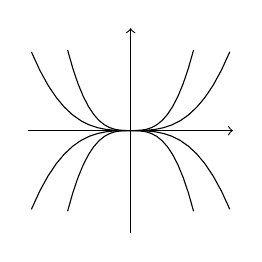
\begin{tikzpicture}
			\draw[->] (-1.3,0) -- (1.3,0);
			\draw[->] (0,-1.3) -- (0,1.3);
			\draw [domain=-1.26:1.26] plot (\x, {0.5*\x^3});
			\draw [domain=-1.26:1.26] plot (\x, {-0.5*\x^3});
			\draw [domain=-0.8:0.8] plot (\x, {2*\x^3});
			\draw [domain=-0.8:0.8] plot (\x, {-2*\x^3});
		\end{tikzpicture}
		\caption*{\(\alpha > 1\)}
	\end{subfigure}%
	\begin{subfigure}{0.25\textwidth}
		\centering
		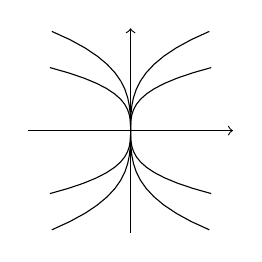
\begin{tikzpicture}
			\draw[->] (-1.3,0) -- (1.3,0);
			\draw[->] (0,-1.3) -- (0,1.3);
			\draw [domain=-1.26:1.26] plot ({0.5*\x^3}, \x);
			\draw [domain=-1.26:1.26] plot ({-0.5*\x^3}, \x);
			\draw [domain=-0.8:0.8] plot ({2*\x^3}, \x);
			\draw [domain=-0.8:0.8] plot ({-2*\x^3}, \x);
		\end{tikzpicture}
		\caption*{\(0 < \alpha < 1\)}
	\end{subfigure}%
	\begin{subfigure}{0.25\textwidth}
		\centering
		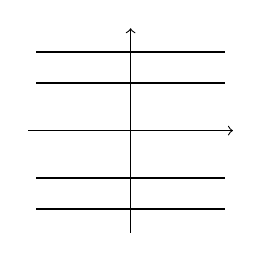
\begin{tikzpicture}
			\draw[->] (-1.3,0) -- (1.3,0);
			\draw[->] (0,-1.3) -- (0,1.3);
			\draw[thick] (-1.2,1) -- (1.2,1);
			\draw[thick] (-1.2,0.6) -- (1.2,0.6);
			\draw[thick] (-1.2,-0.6) -- (1.2,-0.6);
			\draw[thick] (-1.2,-1) -- (1.2,-1);
		\end{tikzpicture}
		\caption*{\(\alpha = 0\)}
	\end{subfigure}%
	\begin{subfigure}{0.25\textwidth}
		\centering
		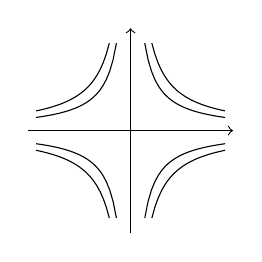
\begin{tikzpicture}
			\draw[->] (-1.3,0) -- (1.3,0);
			\draw[->] (0,-1.3) -- (0,1.3);
			\draw [domain=0.18:1.2] plot (\x, {0.2*\x^(-1)});
			\draw [domain=-1.2:-0.18] plot (\x, {0.2*\x^(-1)});
			\draw [domain=0.18:1.2] plot (\x, {-0.2*\x^(-1)});
			\draw [domain=-1.2:-0.18] plot (\x, {-0.2*\x^(-1)});
			\draw [domain=0.27:1.2] plot (\x, {0.3*\x^(-1)});
			\draw [domain=-1.2:-0.27] plot (\x, {0.3*\x^(-1)});
			\draw [domain=0.27:1.2] plot (\x, {-0.3*\x^(-1)});
			\draw [domain=-1.2:-0.27] plot (\x, {-0.3*\x^(-1)});
		\end{tikzpicture}
		\caption*{\(\alpha < 0\)}
	\end{subfigure}
	\caption{Posibles diagramas de fase de un sistema plano diagonalizable con 
	dos autovalores distintos, dependiendo del parámetro \(\alpha\)}
\end{figure}

\begin{itemize}
	\item Si \(\alpha < 0\), \(\lambda_1\) y \(\lambda_2\) tienen necesariamente
	      signos opuestos. En este caso, el diagrama de fases (o más específicamente, el
	      punto de equilibrio) recibe el nombre de \emph{punto de silla} (piénsese en
	      las curvas de nivel de la función ``silla de montar'' \(z = x^2 - y^2\)).

	\item Si \(\alpha > 0\), \(\lambda_1\) y \(\lambda_2\) tienen el mismo signo.
	      \begin{itemize}
		      \item Si es positivo, al aumentar \(t\) aumenta también la magnitud de la
		            solución, es decir, se aleja (exponencialmente) del origen. Por esto, el
		            diagrama (o el punto de equilibrio) recibe el nombre de \emph{nodo
			            inestable}.
		      \item Si es negativo, al aumentar \(t\) disminuye la magnitud de la solución,
		            es decir, se acerca (exponencialmente) al origen. Por esto, el diagrama (o
		            el punto de equilibrio) recibe el nombre de \emph{nodo estable}.
	      \end{itemize}
	      Hay que mencionar que el origen en sí siempre es una solución estable; estos
	      nombres hacen referencia a lo que ocurre tras una desviación, por pequeña que
	      sea, desde este punto.
\end{itemize}

Los demás casos los veremos con menos detalle, porque las ideas generales son
las mismas para todos y porque éste es el más delicado.

\subsection{Diagonalizable con un autovalor real}

Consideramos el sistema \(y' = \smat{\lambda & \\ & \lambda} y\). La solución
general es
\[\eqsys{
	y_1 = k_1e^{\lambda t} \\
	y_2 = k_2e^{\lambda t}}\]

de donde \(y_1/k_1 = y_2/k_2 > 0\); esta es la ecuación de una semirrecta que
pasa por el origen (de hecho, coincide con el caso límite \(\alpha = 1\) en el
apartado anterior).

\begin{figure}[ht]
	\centering
	\begin{subfigure}{0.5\textwidth}
		\centering
		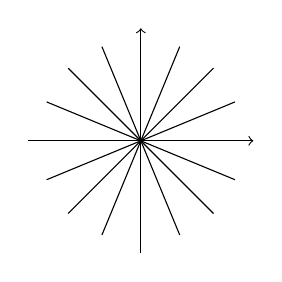
\begin{tikzpicture}[scale=1.3]
			\draw[->] (-1.1,0) -- (1.1,0);
			\draw[->] (0,-1.1) -- (0,1.1);
			\draw (-0.92, -0.38) -- (0.92, 0.38);
			\draw (0.92, -0.38) -- (-0.92, 0.38);
			\draw (-0.71, -0.71) -- (0.71, 0.71);
			\draw (0.71, -0.71) -- (-0.71, 0.71);
			\draw (-0.38, -0.92) -- (0.38, 0.92);
			\draw (0.38, -0.92) -- (-0.38, 0.92);
		\end{tikzpicture}
		\caption*{\(\lambda \neq 0\)}
	\end{subfigure}%
	\begin{subfigure}{0.5\textwidth}
		\centering
		\begin{tikzpicture}[scale=1.3]
			\draw[->] (-1.1,0) -- (1.1,0);
			\draw[->] (0,-1.1) -- (0,1.1);
			\foreach \x in {-0.92, -0.71, -0.38, 0, 0.38, 0.71, 0.92}
			\foreach \y in {-0.92, -0.71, -0.38, 0, 0.38, 0.71, 0.92}
			\fill (\x, \y) circle (0.5pt);
		\end{tikzpicture}
		\caption*{\(\lambda = 0\)}
	\end{subfigure}
	\caption{Posibles diagramas de fase de un sistema plano diagonalizable con 
	un único autovalor, dependiendo del parámetro \(\lambda\)}
\end{figure}

\begin{itemize}
	\item Si \(\lambda > 0\), la solución se aleja (exponencialmente) del origen; el
	      diagrama recibe el nombre de \emph{punto de estrella inestable}. Es un nodo
	      inestable degenerado.
	\item Si \(\lambda < 0\), la solución se acerca (exponencialmente) al origen; el
	      diagrama recibe el nombre de \emph{punto de estrella estable}. Es un nodo
	      estable degenerado.
	\item Si \(\lambda = 0\), la solución es constante para cualquier valor inicial,
	      es decir, el sistema no evoluciona con el tiempo.
\end{itemize}

\subsection{No diagonalizable con un autovalor real}
Consideramos el sistema \(y' = \smat{\lambda & 1 \\ & \lambda}y\), cuya solución
general es
\[
	\begin{cases}
		y_1 = (k_1+k_2t)e^{\lambda t} \\
		y_2 = k_2e^{\lambda t}
	\end{cases}
\]

Si \(\lambda = 0\), esta solución queda reducida a

\[
	\begin{cases}
		y_1 = k_1 + k_2 t \\
		y_2 = k_2
	\end{cases}
\]

La segunda coordenada permanece constante a lo largo del tiempo, mientras que la
primera varía desde \(-\infty\) hasta \(+\infty\) (si \(k_2 > 0\)) o desde
\(+\infty\) hasta \(-\infty\) (si \(k_2 < 0\)).

Si \(\lambda \neq 0\), distinguimos casos en función del valor inicial:

\begin{itemize}
	\item \(k_1 = 0, k_2 = 0\): \(\{(0,0)\}\) es un punto de equilibrio
	\item \(k_1 \neq 0, k_2 = 0\): los dos semiejes de abscisas
	      \(\{(y_1, 0) : y_1 > 0\}\) y \(\{(y_1,0) : y_1 < 0\}\) son trayectorias
	\item Si \(k_2 \neq 0\), podemos despejar \(t\) de \(y_2 = k_2e^{\lambda t}\) como
	      \[t = \frac{1}{\lambda} \log \frac{y_2}{k_2}.\]

	      Sustituyendo en \(y_1 = (k_1 + k_2t)e^{\lambda t}\), obtenemos una ecuación
	      implícita para la trayectoria:
	      \[y_1 = y_2 \left( \frac{k_1}{k_2} + \frac{1}{\lambda} \log \frac{y_2}{k_2}
		      \right).\]

	      Derivando implícitamente se obtiene
	      \(\frac{\dif y_1}{\dif y_2} = \frac{\lambda y_1 + y_2}{\lambda y_2}\); esto
	      quiere decir que, a lo largo de la recta \(\{y_2 = -\lambda y_1\}\), esta
	      derivada se anula y, por tanto, las trayectorias tienen en esa recta tangente
	      vertical.
\end{itemize}

Juntándolo todo, los diagramas de fase son

\begin{figure}[ht]
	\centering
	\begin{subfigure}{0.33\textwidth}
		\centering
		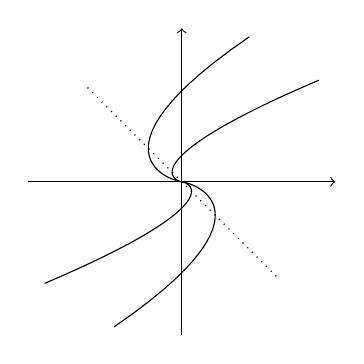
\begin{tikzpicture}[scale=1.5]
			\draw[->] (-1.3,0) -- (1.3,0);
			\draw[->] (0,-1.3) -- (0,1.3);
			\draw[samples=100, domain = -10:-0.15] plot ({(1.5 + \x)*exp(\x)}, {exp(\x)});
			\draw[samples=100, domain = -10:-0.15] plot ({(-1.5 - \x)*exp(\x)}, {-exp(\x)});
			\draw[samples=100, domain = -10:-0.2] plot ({(1 + 1.5*\x)*exp(\x)}, {1.5*exp(\x)});
			\draw[samples=100, domain = -10:-0.2] plot ({(-1 - 1.5*\x)*exp(\x)}, {-1.5*exp(\x)});
			\draw[thin, dotted] (0.8, -0.8) -- (-0.8, 0.8);
		\end{tikzpicture}
		\caption*{\(\lambda > 0\)}
	\end{subfigure}%
	\begin{subfigure}{0.33\textwidth}
		\centering
		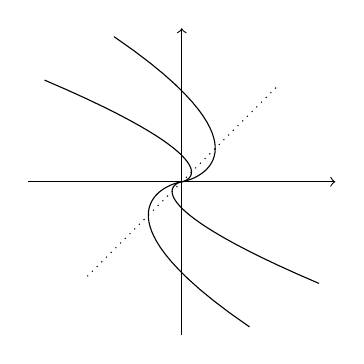
\begin{tikzpicture}[scale=1.5]
			\draw[->] (-1.3,0) -- (1.3,0);
			\draw[->] (0,-1.3) -- (0,1.3);
			\draw[samples=100, domain = 0.15:10] plot ({(1.5 - \x)*exp(-\x)}, {-exp(-\x)});
			\draw[samples=100, domain = 0.15:10] plot ({(-1.5 + \x)*exp(-\x)}, {exp(-\x)});
			\draw[samples=100, domain = 0.2:10] plot ({(1 - 1.5*\x)*exp(-\x)}, {-1.5*exp(-\x)});
			\draw[samples=100, domain = 0.2:10] plot ({(-1 + 1.5*\x)*exp(-\x)}, {1.5*exp(-\x)});
			\draw[thin, dotted] (-0.8, -0.8) -- (0.8, 0.8);
		\end{tikzpicture}
		\caption*{\(\lambda < 0\)}
	\end{subfigure}%
	\begin{subfigure}{0.33\textwidth}
		\centering
		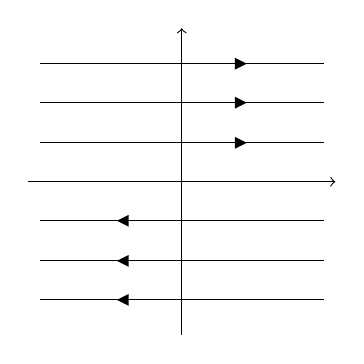
\begin{tikzpicture}[scale=1.5]
			\draw[->] (-1.3,0) -- (1.3,0);
			\draw[->] (0,-1.3) -- (0,1.3);
			\foreach \y in {1, 0.67, 0.33}
				{
					\draw (-1.2,\y) -- (1.2,\y);
					\fill (0.55, \y) -- (0.45, \y-0.05) -- (0.45, \y+0.05) -- cycle;
				}
			\foreach \y in {-0.33, -0.67, -1}
				{
					\draw (-1.2,\y) -- (1.2,\y);
					\fill (-0.55, \y) -- (-0.45, \y+0.05) -- (-0.45, \y-0.05) -- cycle;
				}
		\end{tikzpicture}
		\caption*{\(\lambda = 0\)}
	\end{subfigure}
	\caption{Posibles diagramas de fase de un sistema plano no diagonalizable con 
	un único autovalor real, dependiendo del parámetro \(\lambda\)}
\end{figure}

Como siempre, el comportamiento es distinto en función del signo de \(\lambda\):

\begin{itemize}
	\item Si \(\lambda > 0\), la solución se aleja exponencialmente del origen. En
	      este caso, el diagrama se llama \emph{nodo impropio inestable}.
	\item Si \(\lambda < 0\), la solución se acerca exponencialmente al origen. En
	      este caso, el diagrama se llama \emph{nodo impropio estable}.
\end{itemize}

\subsection{No diagonalizable con dos autovalores complejos conjugados}
Consideramos el sistema \(y' = \smat{a & b \\ -b & a}y\), que tiene por solución
general

\[
	\begin{cases}
		y_1 = e^{at}(k_1 \cos bt + k_2 \sin bt) \\
		y_2 = e^{at}(-k_1 \sin bt + k_2 \cos bt)
	\end{cases}
\]

Definimos \(r_0^2 = k_1^2+k_2^2\) y \(\theta_0 \in \R\) tal que
\[\cos \theta_0 = \frac{k_1}{r_0} \qquad \text{y} \qquad \sin \theta_0 = \frac{k_2}{r_0}.\]
Se puede comprobar que así la solución general toma la forma
\[
	\begin{cases}
		y_1 = r_0e^{at} \cos (\theta_0 - bt) \\
		y_2 = r_0e^{at} \sin (\theta_0 - bt)
	\end{cases}
\]

y, definiendo \(r(t) = r_0e^{at}\) y \(\theta(t) = \theta_0 - bt\), se tiene
\[
	\begin{cases}
		y_1 = r(t) \cos \theta(t) \\
		y_2 = r(t) \sin \theta(t)
	\end{cases}
\]
con lo que queda descrito el camino \(t \mapsto \smat{y_1(t) \\ y_2(t)}\) en
coordenadas polares.

\begin{itemize}
	\item Si \(a = 0\), entonces \(r(t) \equiv r_0\), es decir, las trayectorias son
	      circunferencias de radio \(r_0\). El diagrama recibe el nombre de \emph{centro}.
	\item Si \(a \neq 0\), entonces las trayectorias son \emph{espirales logarítmicas}
	      \begin{itemize}
		      \item Si \(\lambda > 0\), las soluciones se alejan exponencialmente del
		            origen. En este caso, el diagrama recibe el nombre de \emph{foco inestable}.
		      \item Si \(\lambda < 0\), las soluciones se acercan exponencialmente al
		            origen. En este caso, el diagrama recibe el nombre de \emph{foco estable}.
	      \end{itemize}
\end{itemize}

\begin{figure}[ht]
	\centering
	\begin{subfigure}{0.5\textwidth}
		\centering
		\begin{tikzpicture}[scale=0.7]
			\draw[->] (-3,0) -- (3,0);
			\draw[->] (0,-3) -- (0,3);
			\draw [samples=100, domain = -10:1] plot ({exp(\x)*cos(-\x r)},{exp(\x)*sin(-\x r)});
			\draw [samples=100, domain = -10:1] plot ({exp(\x)*cos((2-\x) r)},{exp(\x)*sin((2-\x) r)});
			\draw [samples=100, domain = -10:1] plot ({exp(\x)*cos((4-\x) r)},{exp(\x)*sin((4-\x) r)});
		\end{tikzpicture}
		\caption*{\(a \neq 0\)}
	\end{subfigure}%
	\begin{subfigure}{0.5\textwidth}
		\centering
		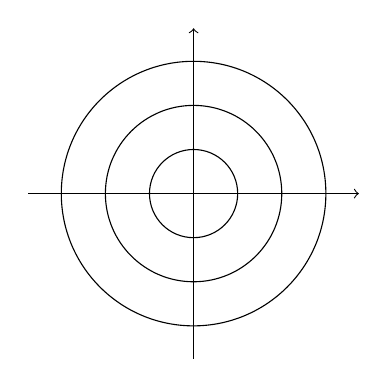
\begin{tikzpicture}[scale=0.7]
			\draw[->] (-3,0) -- (3,0);
			\draw[->] (0,-3) -- (0,3);
			\draw (0,0) circle (0.8);
			\draw (0,0) circle (1.6);
			\draw (0,0) circle (2.4);
		\end{tikzpicture}
		\caption*{\(a = 0\)}
	\end{subfigure}
	\caption{Posibles diagramas de fase de un sistema plano no diagonalizable con 
	dos autovalores complejos conjugados, dependiendo del parámetro \(a\)}
\end{figure}

\subsection{Deshacer el cambio}
Habíamos hecho el cambio de variable \(y = P^{-1}x\) para resolver el sistema
\(x' = Ax = (PBP^{-1})x\). Ahora lo deshacemos: \(x = Py = \smat{v_1 & v_2}
\smat{y_1 \\ y_2}\).

Como ya sabemos de Álgebra Lineal, la transformaciones lineales
\(\R^2 \to \R^2\) no singulares deforman, rotan o hacen reflexiones sobre el
plano. Estas transformaciones quedan completamente determinadas por las imágenes de
dos vectores linealmente independientes, que en nuestro caso son \(e_1 = \smat{1
	\\ 0}\) y \(e_2 = \smat{0 \\ 1}\).

\(P\) es la \emph{única} transformación lineal que lleva \(e_1 \mapsto v_1\) y
\(e_2 \mapsto v_2\). Por tanto, para obtener el diagrama de fase de \(x' = Ax\),
basta transformar el de \(y' = By\) de forma que sea compatible con las
transformaciones
\[e_1 \mapsto v_1 \qquad e_2 \mapsto e_2.\]

\section{Oscilaciones mecánicas}

Para terminar con el capítulo, veamos cómo se puede aplicar lo que hemos visto a
la modelización de las \emph{oscilaciones mécanicas} y, de hecho, a muchos otros
fenómenos.

Como vamos a ver, las oscilaciones mecánicas se pueden modelizar con ecuaciones
diferenciales lineales de segundo orden con coeficientes constantes; además,
cualquier ecuación diferencial tal modela un sistema físico que presenta
``oscilaciones'' en algún sentido, por lo que no perdemos generalidad al
restringirnos a este caso. Esto ayuda a tener una intuición física de cómo se
comporta el sistema.

Consideramos un objeto de masa \(m\) suspendido del techo mediante un muelle,
como se muestra en la figura~\ref{fig:muelle}. El sistema de referencia está
elegido de tal manera que \(x=0\) corresponde con la posición de equilibrio de
la masa.

\begin{figure}[ht]
	\centering
	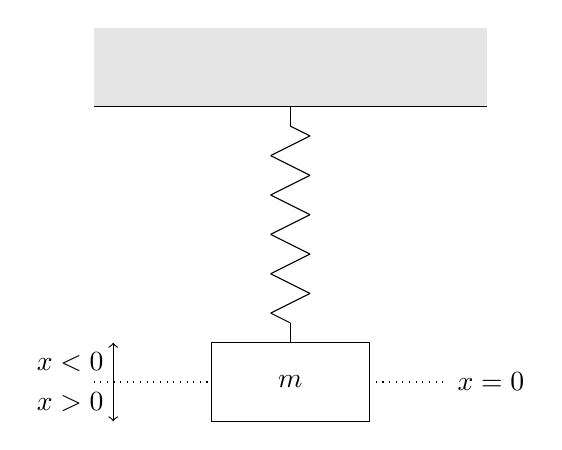
\begin{tikzpicture}[scale=0.5]
		\fill[color=gray!20] (-5,10) rectangle (5,8);
		\draw (-5,8) -- (5,8);
		\draw (0,8) -- (0,7.5);
		\draw (0,7.5) -- (0.5,7.25);
		\draw (0.5,7.25) -- (-0.5,6.75);
		\draw (-0.5,6.75) -- (0.5,6.25);
		\draw (0.5,6.25) -- (-0.5,5.75);
		\draw (-0.5,5.75) -- (0.5,5.25);
		\draw (0.5,5.25) -- (-0.5,4.75);
		\draw (-0.5,4.75) -- (0.5,4.25);
		\draw (0.5,4.25) -- (-0.5,3.75);
		\draw (-0.5,3.75) -- (0.5,3.25);
		\draw (0.5,3.25) -- (-0.5,2.75);
		\draw (-0.5,2.75) -- (0,2.5);
		\draw (0,2) -- (0,2.5);
		\draw (-2,2) rectangle (2,0);
		\node at (0,1) {\(m\)};
		\draw[dotted] (-5,1) -- (-2,1);
		\draw[->] (-4.5,1) -- node[left,midway] {\(x < 0\)}(-4.5,2);
		\draw[->] (-4.5,1) -- node[left,midway] {\(x > 0\)}(-4.5,0);
		\draw[dotted] (2,1) -- (4,1) node[right] {\(x = 0\)};
	\end{tikzpicture}
	\caption{Masa colgada de un muelle}
	\label{fig:muelle}
\end{figure}

Según la segunda ley de Newton, \(\sum_i F_i = mx''\). Las fuerzas que actúan sobre
la masa son

\begin{itemize}
	\item la gravedad, en sentido positivo, de módulo \(mg\)
	\item la fuerza de recuperación del muelle, en sentido opuesto al
	      desplazamiento, de módulo \(|kx|\), siendo \(k \geq 0\) la \emph{constante de
		      recuperación del muelle}
	\item la fuerza de rozamiento o amortiguación, en sentido opuesto a la
	      velocidad, de módulo \(|cx'|\), siendo \(c \geq 0\) la \emph{constante de rozamiento}
	\item una fuerza externa \(b(t)\)
\end{itemize}

Por tanto, la ecuación diferencial que modela este sistema es
\begin{equation} \label{eq:osc1}
	mx'' = mg - kx - cx' + b(t)
\end{equation}

\begin{remark}
	La hipótesis de que \(k\) y \(c\) son constantes es razonable. La hipótesis de
	linealidad de la ecuación es algo más atrevida, pero observaciones empíricas
	justifican esta elección de las fuerzas de recuperación y rozamiento.
\end{remark}

Para analizar la ecuación~\eqref{eq:osc1}, suponemos que \(m=1\) e incluimos la
fuerza de la gravedad en la fuerza externa, de forma que queda
\begin{equation} \label{eq:osc2}
	x'' = - kx - cx' + b(t)
\end{equation}

\begin{remark}
	Esta es la ecuación diferencial lineal de orden 2 más general tal que su
	homogénea asociada tiene coeficientes constantes (e.d. la ecuación diferencial
	lineal de orden 2 más general que sabemos resolver).
\end{remark}

La ecuación homogénea asociada a~\eqref{eq:osc2} es
\begin{equation} \label{eq:osch}
	x'' = - cx' - kx \iff x'' + cx' + kx = 0
\end{equation}

Introduciendo las variables \(x_1 = x\) y \(x_2 = x'\), tenemos que el sistema
\(2 \times 2\) asociado es
\[\mat{x_1' \\ x_2'} = \mat{0 & 1 \\ -k & -c} \mat{x_1 \\ x_2} \iff
	\left\{\begin{array}{c c c c}
		x_1' & = &       & x_2   \\
		x_2' & = & -kx_1 & -cx_2
	\end{array}\right.
\]

La matriz del sistema tiene por polinomio característico
\[
	p(\lambda) =
	\begin{vmatrix}
		-\lambda & 1 \\ -k & -c-\lambda
	\end{vmatrix} =
	\lambda(\lambda + c) + k = \lambda^2 + c\lambda + k
\]
\begin{remark}
	El polinomio característico (y por tanto los autovalores) se puede obtener
	directamente a partir de la ecuación homogénea~\eqref{eq:osch}: \(x'' + cx' +
	kx = 0 \leftrightarrow \lambda^2 + c\lambda + k = 0\).
\end{remark}

Tenemos entonces que los autovalores de la matriz del sistema son
\[\lambda_1 = \frac{-c + \sqrt{c^2 - 4k}}{2}, \quad \lambda_2 = \frac{-c - \sqrt{c^2-4k}}{2}\]

Vamos a empezar resolviendo casos particulares sencillos, para ir complicando el
problema poco a poco hasta llegar al caso general.

\subsection{Movimiento oscilatorio armónico}
Este es el caso (mínimamente interesante) más sencillo, en el que no hay
amortiguación ni fuerzas externas, es decir, \(c = 0, b(t) = 0\).

Con estas simplificaciones, la ecuación queda reducida a \(x'' = -kx\), y los
autovalores son \(\pm i\sqrt{k}\). El valor \(\omega_0 = \sqrt{k}\) recibe el
nombre de \emph{frecuencia fundamental} del sistema.

La matriz \(B\) asociada es, por tanto, \(B = \smat{0 & \omega_0 \\ -\omega_0 &
	0}\), y su exponencial es \(e^{Bt} = \smat{\cos \omega_0 t & \sin \omega_0 t
	\\ -\sin \omega_0 t & \cos \omega_0 t}\). Así, la solución general del sistema
es
\[\mat{x_1 \\ x_2} = P \mat{\cos \omega_0 t & \sin \omega_0 t
		\\ -\sin \omega_0 t & \cos \omega_0 t}\mat{c_1 \\ c_2} = \mat{p_{11} & p_{12} \\
		p_{21} & p_{22}} \mat{c_1 \cos \omega_0 t + c_2 \sin \omega_0 t \\ -c_1 \sin
		\omega_0 t + c_2 \cos \omega_o t}\]
y la solución de la ecuación de orden 2 es
\begin{align*}
	x = x_1 & = p_{11}c_1 \cos \omega_0 t + p_{11}c_2 \sin \omega_0 t - p_{12}c_1
	\sin \omega_0 t + p_{12}c_2 \cos \omega_0 t                                   \\
	        & = \underbrace{(p_{11}c_1+p_{12}c_2)}_{k_1} \cos \omega_0 t +
	\underbrace{(p_{11}c_2 - p_{12}c_1)}_{k_2} \sin \omega_0 t = k_1 \cos \omega_0
	t + k_2 \sin \omega_0 t
\end{align*}

\begin{remark}
	En realidad, esto se podía haber deducido directamente de la solución general
	del sistema, porque sabemos de la teoría general que el conjunto de soluciones
	es un espacio vectorial de dimensión 2 y, en este caso, cada solución
	particular debe ser combinación lineal de
	\(\{\cos \omega_0 t, \sin \omega_0 t\}\), que son linealmente independientes,
	así que debe ser de la forma \(k_1 \cos \omega_0 t + k_2 \sin \omega_0 t\).
\end{remark}

Tomando \(r_0 = \sqrt{k_1^2+k_2^2}\) y \(\theta_0 \in \R\) tal que \(r_0 \cos
\theta_0 = k_1\) y \(r_0 \sin \theta_0\), nos queda
\[r_0 \cos (\omega_0 t - \theta_0) = r_0(\cos \omega_0 t \cos \theta_0 + \sin
	\omega_0 t \sin \theta_0) = k_1 \cos \omega_0 t + k_2 \sin \omega_0 t\]

En resumen, la masa oscilará sinusoidalmente con un periodo de \(T =
\frac{2\pi}{\omega_0}\) y el diagrama es el de un centro.

\subsection{Movimiento oscilatorio amortiguado}
Introducimos ahora una amortiguación, de forma que la ecuación queda
\(x'' = - cx' - kx\). Los autovalores son \(\frac{1}{2}(-c \pm \sqrt{c^2-4k})\), así
que distinguimos casos en función del valor de \(c^2-4k\):
\begin{itemize}
	\item \(c^2-4k > 0\) (caso \emph{sobreamortiguado}): se tienen dos autovalores
	      reales distintos, ambos negativos:
	      \[\lambda_1 = \frac{-c + \sqrt{c^2-4k}}{2}, \quad \lambda_2 = \frac{-c -
			      \sqrt{c^2-4k}}{2}.\]
	      La solución general del sistema asociado es
	      \[\mat{x_1 \\ x_2} = P \mat{e^{\lambda_1 t} & 0 \\ 0 & e^{\lambda_2 t}} \mat{c_1
			      \\ c_2};\]
	      razonando como en la observación anterior, la solución de la ecuación de
	      orden 2 es
	      \[x = x_1 = k_1e^{\lambda_1 t} + k_2e^{\lambda_2 t}\]
	      Como los autovalores son negativos, el diagrama de fases es el de un nodo
	      estable. Además, \(x(t) \to 0\) exponencialmente rápido. La gráfica de la
	      solución puede tomar tres formas distintas:
	      \begin{figure}[ht]
		      \centering
		      \begin{subfigure}{0.33\textwidth}
			      \centering
			      \begin{tikzpicture}
				      \draw[->] (-0.5,0) -- (3,0);
				      \draw[->] (0,-1) -- (0,2);
				      \draw [domain=0:2.8] plot (\x, {0.7*exp(-\x)+exp(-2*\x)});
			      \end{tikzpicture}
		      \end{subfigure}%
		      \begin{subfigure}{0.33\textwidth}
			      \centering
			      \begin{tikzpicture}
				      \draw[->] (-0.5,0) -- (3,0);
				      \draw[->] (0,-1) -- (0,2);
				      \draw [domain=0:2.8, samples=50] plot (\x, {5*exp(-\x)-4*exp(-2*\x)});
			      \end{tikzpicture}
		      \end{subfigure}%
		      \begin{subfigure}{0.33\textwidth}
			      \centering
			      \begin{tikzpicture}
				      \draw[->] (-0.5,0) -- (3,0);
				      \draw[->] (0,-1) -- (0,2);
				      \draw [domain=0:2.8, samples=50] plot (\x, {-4*exp(-\x)+5*exp(-2*\x)});
			      \end{tikzpicture}
		      \end{subfigure}
			\caption{Posibles gráficas con respecto al tiempo de un objeto que
			  sigue un movimiento armónico, caso sobreamortiguado}
	      \end{figure}

	      En particular, la amortiguación es demasiado grande para que haya
	      oscilaciones. Si las condiciones iniciales son demasiado extremas (mucho
	      desplazamiento o velocidad muy grande), puede parecer que la masa va a
	      oscilar; sin embargo, rápidamente se estabiliza.
	\item \(c^2 - 4k < 0\) (caso \emph{subamortiguado}): se tienen dos autovalores
	      complejos:
	      \[\lambda_1 = -\frac{c}{2}+i\sqrt{k-\left(\frac{c}{2}\right)^2} = a + bi, \quad
		      \lambda_2 = -\frac{c}{2}-i\sqrt{-k\left(\frac{c}{2}\right)^2} = a - bi\]

	      La solución general del sistema asociado es
	      \[\mat{x_1 \\ x_2} = P \mat{e^{at} \cos bt & e^{at} \sin bt \\ -e^{at} \sin
		      bt & e^{at} \cos bt} \mat{c_1 \\ c_2}\]
	      y, procediendo como antes, la solución de la ecuación de orden 2 es
	      \[x = x_1 = k_1e^{at} \cos bt + k_2e^{at} \sin bt.\]
	      Tomando \(r_0 = \sqrt{k_1^2+k_2^2}\) y \(\theta_0 \in \R\) tal que \(r_0
	      \cos bt = k_1\) y \(r_0 \sin bt = k_2\), nos queda
	      \[x = r_0e^{at} \cos (bt - \theta_0),\]
	      siendo \(a = -c/2 < 0\). El diagrama de fases es ahora el de un foco
	      estable, y la gráfica de la solución tiene esta forma:
	      \begin{figure}[ht]
		      \centering
		      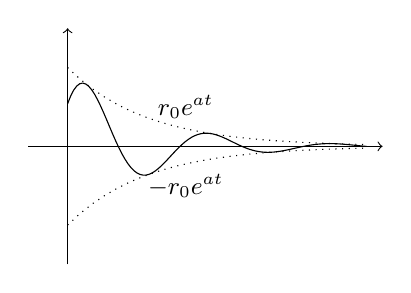
\begin{tikzpicture}
			      \draw[->] (-0.5,0) -- (4,0);
			      \draw[->] (0,-1.5) -- (0,1.5);
			      \draw [domain = 0:3.8, samples=100] plot (\x, {exp(-\x)*cos((4*\x-1) r)});
			      \draw [domain = 0:3.8, dotted] plot (\x, {exp(-\x)});
			      \draw [domain = 0:3.8, dotted] plot (\x, {-exp(-\x)});
			      \node at (1.5,0.5) {\small\(r_0e^{at}\)};
			      \node at (1.5,-0.5) {\small\(-r_0e^{at}\)};
		      \end{tikzpicture}
			\caption{Posibles gráficas con respecto al tiempo de un objeto que
			  sigue un movimiento armónico, caso subamortiguado}
	      \end{figure}

	      En este caso sí que hay oscilaciones, aunque decaen a 0 exponencialmente rápido.

	\item \(c^2-4k=0\) (caso \emph{críticamente amortiguado}): ahora hay un único
	      autovalor real, \(\lambda = -c/2\), de multiplicidad algebraica 2 y
	      multiplicidad geométrica 1, puesto que
	      \[\mat{0 & 1 \\ -k & -c} - \mat{\lambda & 0 \\ 0 & \lambda} = \mat{c/2 & 1
			      \\ -k & -c/2}\]
	      es una matriz de rango 1.

	      La solución general del sistema es
	      \[\mat{x_1 \\ x_2} = e^{\lambda t} P \mat{1 & t \\ 0 & 1} \mat{c_1 \\
			      c_2},\]
	      con lo que el diagrama de fases es el de un nodo impropio estable y la
	      solución de la ecuación de orden 2 es de la forma
	      \[x = x_1 = e^{\lambda t}(k_1 + k_2t).\]
	      La gráfica puede tomar tres formas distintas:
	      \begin{figure}[ht]
		      \centering
		      \begin{subfigure}{0.33\textwidth}
			      \centering
			      \begin{tikzpicture}[scale=0.67]
				      \draw[->] (-0.5,0) -- (4,0);
				      \draw[->] (0,-0.5) -- (0,3);
				      \draw [domain=0:3.7] plot (\x, {exp(-\x)*(2+\x)});
			      \end{tikzpicture}
		      \end{subfigure}%
		      \begin{subfigure}{0.33\textwidth}
			      \centering
			      \begin{tikzpicture}[scale=0.67]
				      \draw[->] (-0.5,0) -- (4,0);
				      \draw[->] (0,-0.5) -- (0,3);
				      \draw [domain=0:3.7, samples=50] plot (\x, {exp(-\x)*(2+5*\x)});
			      \end{tikzpicture}
		      \end{subfigure}%
		      \begin{subfigure}{0.33\textwidth}
			      \centering
			      \begin{tikzpicture}[scale=0.67]
				      \draw[->] (-0.5,0) -- (4,0);
				      \draw[->] (0,-0.5) -- (0,3);
				      \draw [domain=0:3.7, samples=50] plot (\x, {exp(-\x)*(2-\x)});
			      \end{tikzpicture}
		      \end{subfigure}
			\caption{Posibles gráficas con respecto al tiempo de un objeto que
			  sigue un movimiento armónico, caso críticamente amortiguado}
	      \end{figure}

	      Como se puede apreciar, el caso críticamente amortiguado se comporta igual,
	      cualitativamente, que el sobreamortiguado; en particular, ahora tampoco hay
	      oscilaciones de ningún tipo.
\end{itemize}

\subsection{Caso general}
Consideramos, para finalizar, el caso en que existe una fuerza externa
\(b(t) \not \equiv 0\). Como ya sabemos, la solución general del caso no
homogéneo es \(x(t) = x_h(t) + x_p(t)\), siendo \(x_h(t)\) la solución general
de la ecuación homogénea y \(x_p(t)\) una solución particular de la ecuación
no homogénea. Como ya hemos visto, en cualquier caso con amortiguación
\(x_h(t) \to 0\) exponencialmente rápido y, por tanto, el comportamiento a
largo plazo del sistema es el de \(x_p(t)\).

Vamos a estudiar dos casos de interés especial:

\begin{itemize}
	\item \(b(t) \equiv g\), es decir, sólo existe la fuerza de la gravedad. En
	      este caso, una solución particular es la solución constante \(x_p(t) \equiv
	      \frac{g}{k}\) y, por tanto, la solución general es \(x(t) = x_h(t) +
	      \frac{g}{k}\). Esta solución es la misma que en el caso homogéneo, solo que
	      la posición de equilibrio se desplaza de \(x=0\) a \(x=\frac{g}{k}\) por
	      efecto de la gravedad.
	\item La fuerza externa es periódica, de la forma
	      \(b(t) = F_0 \cos \omega t\). \(F_0\) es la \emph{amplitud} de la fuerza y
	      \(\omega\) es la \emph{frecuencia} con la que se ejerce.

	      Es razonable conjeturar una solución particular de la forma \(x_p(t) =
	      \alpha \cos (\omega t - \beta)\). De hecho, se obtiene que \(x_p\) así
	      definida es solución para los valores de los parámetros
	      \[\alpha = \frac{F_0}{\sqrt{(\omega_0^2-\omega^2)^2+c^2\omega^2}} \quad
		      \text{y} \quad \beta \in \R \text{ tal que }
		      \begin{cases}
			      \cos \beta =
			      \frac{\omega_0^2-\omega^2}{\sqrt{(\omega_0^2-\omega^2)^2+c^2\omega^2}} \\
			      \sin \beta = \frac{c\omega}{\sqrt{(\omega_0^2-\omega^2)^2+c^2\omega^2}}
		      \end{cases}
	      \]

	      siendo \(\omega_0 = \sqrt{k}\) la frecuencia fundamental definida
	      anteriormente.

	      En estas condiciones puede aparecer el fenómeno de \emph{resonancia},
	      consistente en que las oscilaciones son mucho mayores de lo que serían en
	      ausencia de una fuerza externa y mucho mayores que la amplitud de la fuerza
	      externa \(F_0\):

	      Si \(\omega \approx \omega_0\), entonces \(\omega_0^2-\omega^2 \approx 0\),
	      con lo que \(\alpha \approx \frac{F_0}{c\omega}\). En particular, si
	      \(c \approx 0\) (i.e. hay muy poca amortiguación), entonces \(\alpha\) (la
	      amplitud de las \emph{oscilaciones}) puede ser enorme aunque \(F_0\) (la
	      amplitud de la \emph{fuerza externa}) sea pequeña.

	      El fenómeno de resonancia es el responsable del colapso de numerosos puentes
	      y estructuras similares, debido a fuerzas externas con una frecuencia
	      peligrosamente cercana a la de la estructura. Esta fuerza puede ser debida
	      al viento\footnote{\url{https://archive.org/details/CEP176}}, a los pasos
	      sincronizados de gente caminando por
	      encima\footnote{\url{https://youtu.be/2cuXbpXRvJ0}}, etc.
\end{itemize}

\end{document}
